\section{Weitere Anwendung mit Bluemix}

Da die Aufgabe explizit WordPress nennt, haben wir uns zuerst dies angesehen.
Es stellte sich heraus, dass WordPress einst nicht ganz simpel auf Bluemix zu nutzen war, was zum einen an einer Art fehlendem, fertigen LAMP Stack lag, zum anderen an einer nicht existenten, persistenten Dateispeichermöglichkeit in Bluemix.

Dies hat sich jedoch geändert und WordPress lässt sich seit letztem Dezember nun enorm simpel in Bluemix aufsetzen.
Es sind essentiell nur noch wenige Klicks in der grafischen Oberfläche notwendig, was wir so auch erfolgreich durchführten.
Realisiert wird dies mittels eines sogenannten \enquote{Boilerplate} Pakets, welches praktisch ein Set an Services beinhaltet. Abbildung \ref{fig:wpbluemix} zeigt die Übersicht der laufenden Anwendungen und Dienste, die untere Anwendung und die unteren drei Dienste werden beim Ausbringen des Boilerplate Pakets erzeugt.
Es werden darüber hinaus Plugins angeboten, die eine Verknüpfung von Wordpress mit beispielsweise IBM Object Storage ermöglicht, um Mediadaten persistent zu speichern. Unsere WordPress-Instanz ist unter \url{http://wpcloud.mybluemix.net/} zu erreichen.

\begin{figure}
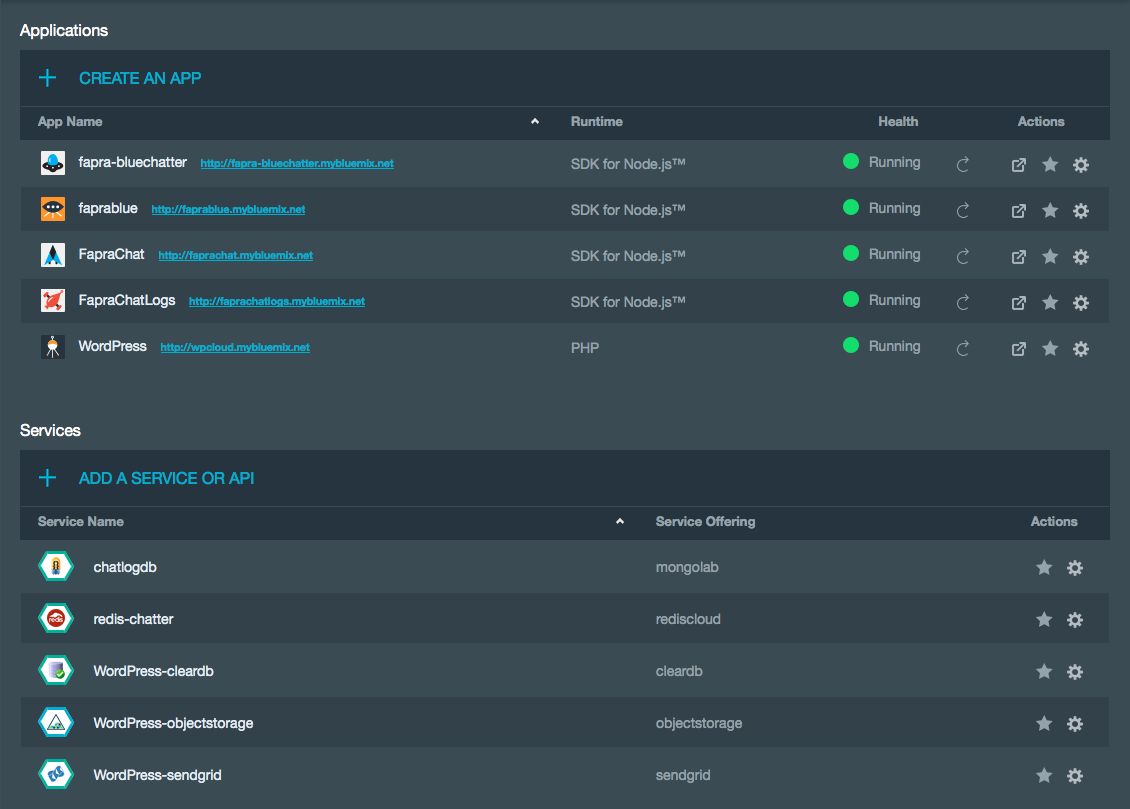
\includegraphics[width=\linewidth]{WordPress.png}
\caption{Laufende Anwendungen und Dienste in Bluemix}
\label{fig:wpbluemix}
\end{figure}

Anschließend widmeten wir uns den beiden genannten Beispielanwendungen.
Da \enquote{todo-apps} auf den ersten Blick eine ähnliche Komplexität wie WordPress aufzuweisen scheint (es kommt mit fertigen Deployment-Skripten), haben wir folgend \enquote{bluechatter} deployed.

Dazu wurde das Script \texttt{deploy-bluechatter.sh} genutzt.
Dieses startet nach dem Login einen Redis Datenbankservice, klont das bluechatter Respository und pusht dieses, nach einer kleinen Modifikation des Redis "Plans" (der im Originalrepo genutzte existiert nicht mehr), zu Bluemix.

Weitere Befehle, wie in 4.3, sind nicht notwendig, da die Relationen und Konfigurationen des/der Service(s) und Application(s) in der \texttt{manifest.yml} bereits definiert sind.
Dieser Ansatz der Konfiguration empfielt sich im allgemeinen für "Echtwelt"-Projekte, speziell wenn die Konfiguration (ver|ge)teilt werden können soll. Der so deployte Chat kann unter \url{http://fapra-bluechatter.mybluemix.net/} erreicht werden.
